% Chapter Template

\chapter{Design} % Main chapter title

\label{Chapter5} % Change X to a consecutive number; for referencing 

\section{User Interface Design}
This section is divided into two parts, graphics design which will focus on what the user can see and why they displayed in that order, and gesture interaction design which will focus on what gestures the user are able to perform and why this project chooses these gestures.
\subsection{Graphics design}
Because Leap Motion system used the right-handed coordinate system. So, when designing the user interface, this project assumes that most user are right-hander. But if some users are left-hander, this virtual environment should not cause much inconvenience for them. The QR Code is selected as a starter imageTarget for the project. And based on the right handed coordinate system and student survey, this project decides to display the PDF/PPT reader on the right side of desktop which obeys the rule of user friendly. 
\\
\\
Below the PDF/PPT reader there is a ’blackboard’, it is used for displaying the available documents. It saves the space on the desktop and provides a convenient way for user to get access to all the materials. The PDF reader is displayed vertically, and the document list should display horizontal to the desktop rather than vertical to the desktop. The reason is when user is looking at the PDF, their line of sight is horizontal to the desktop. If the document list is vertical to the desktop, the user needs to move their head to check the information. But they are wearing the headset, moving head always means that they will have more possibility to lose track of the imageTarget (imageTarget is on the left side of the PDF reader but if the document list is displayed vertically, it should be on the right side of the PDF reader). So, in order to keep the system more stable (even lose track of the imageTarget will not let the virtual object display, but may still have some possibility to cause a mess). 
\\
\\
On the left side of the desktop, user can place their own physical materials and personal belongs. The laptop which is used as the Leap Motion’s server and the Leap Motion device should be displayed on the right side of the Laptop which fit the right-handed coordinate system. The design of the bulletin board is focused on displaying the simplest thing but needs to remind user very often. So, this project chooses to display weather, temperature, date and tasks. Weather and date information is one of the most significant information everyone wants to check, and putting this information can avoid them to check it on their phone. Listing the tasks in a striking place is a way to improve students study efficiency. Because in the survey, students reflect that when they can see their tasks all the time, they will have a motivation to follow their task and focus their mind. 
\\
\\
The background of the bulletin board is a transparent image. Transparent background can let user be able to see what is behind the bulletin board, and this experience can help user to feel that this object actually immersed in the real world compared with an opaque background. Also, the desktop will display two large digital objects which are bulletin board and PDF reader, if both two are opaque, the view of user will be limited. And they will feel that there is a barrier in front of them which can cause a sense of repression after working in this environment for a long time. The design of the project can be explained like the following figure:
\begin{figure}[h]
    \centering
	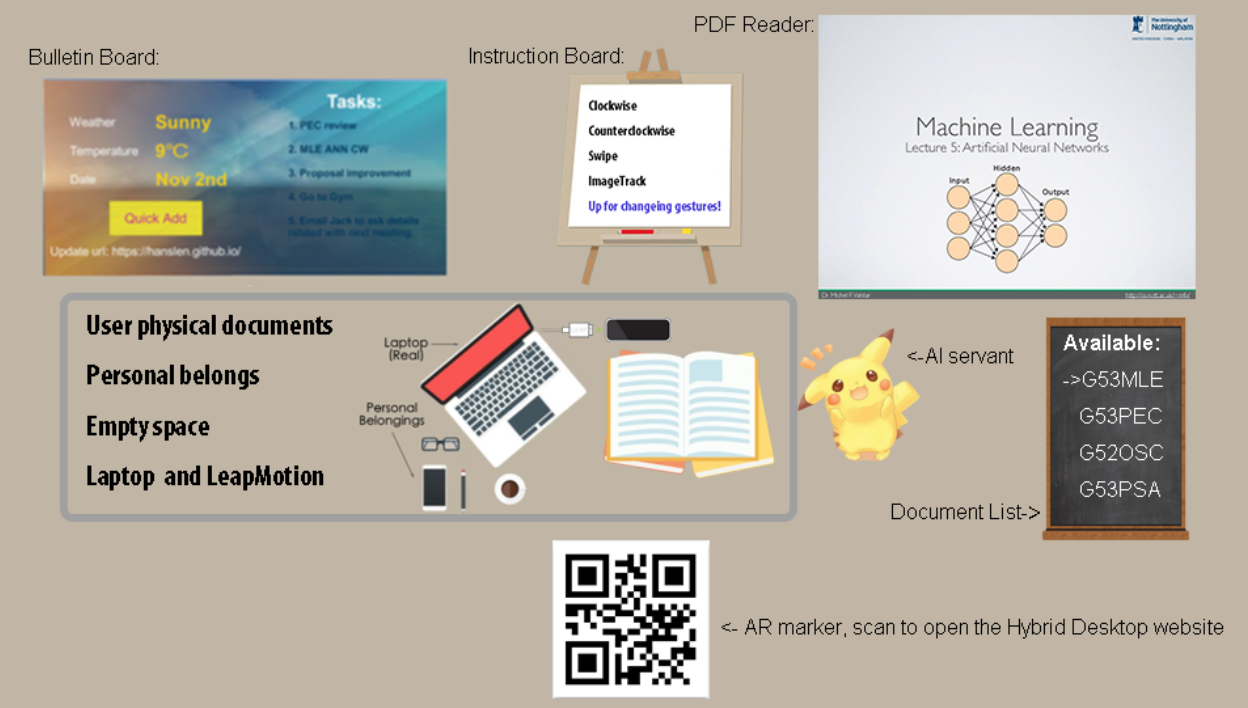
\includegraphics[width=\textwidth]{design}
    \caption{User Interface Design}
    \label{fig:mesh1}
\end{figure}
\subsection{Gesture interaction design}
This application will be used for university students and its main goal is to help with their studying habit, so the gestures should be easy to perform and their meaning should be highly matched with the performance. Then, it needs to define the possible gestures which can be recognized by Leap Motion, because easy and simple gesture recognition rate is much greater than complex gestures. Some scenes are imaged: When people are performing zoom in or zoom out command, there are two usual gesture:\\ 1. Using thumb and index finger to perform a stretching gesture for zooming out, and shrinking gesture for zooming in. \\2. To do a clockwise gesture. \\Compared with finger interaction, the application prefers hand interaction. Because the size of finger is much smaller than hand, so the capture of data will be less accurate. Also, in the Leap Motion’s API, it has the gesture recognition for clock wise. So this application defines that clockwise gesture can be used for controlling the size of PDF reader. 
\\
\\
Another import control of the PDF reader is switching the PDF to the next page or back to the previous one. The most natural way to do this command is the swipe gesture. It is not complex to implement, the Leap Motion device can get the hand position, by analyzing the movement of hand, the application will be able to recognize these gestures. But for switching the PDF, when asking people which gesture they usually use for switching the PDF, they will have no idea. Because in real world, there is always a button for switching the PDF. So based on the user experience, the project defines a virtual button for doing this switching command, and the gesture for user is hovering their hand over this button. 
\section{System Structure design}
In this section, it will discuss the project’s framework design and the database design. Graphs will be used to illustrate the relationship between each component. 
\subsection{Framework design}
There are three basic components of the project’s framework one imageTarget for all digital objects, another imageTarget for annotation box and a Leap Motion Client Game Object. The following figure is the design of the framework, the round rectangular stands for the basic components and each ellipse stands for a digital object, and the rhombus stand for the backend action.
\\
\begin{figure}[h]
    \centering
	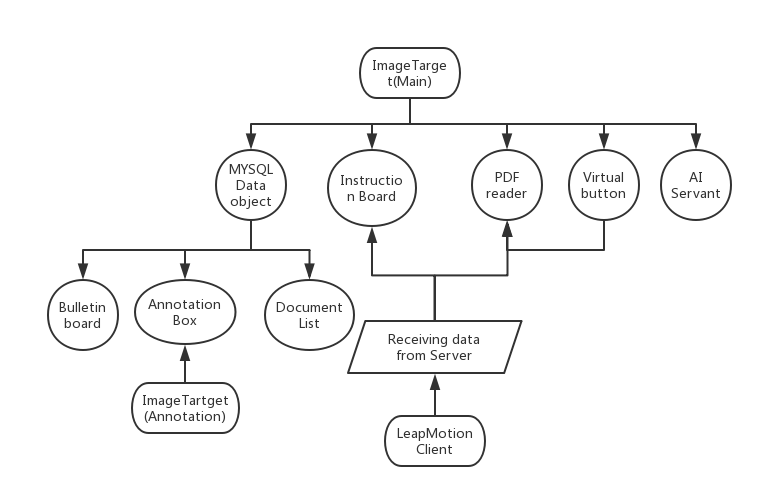
\includegraphics[width=\textwidth]{dt_design}
    \caption{Hybrid desktop framework design}
    \label{fig:mesh1}
\end{figure}
\\
ImageTarget is the foundation of the project, and all the digital objects should belong to it and inherit its properties. What needs to be explained in special is the Annotation Box, it does not only belong to the ImageTarget(Main), and belongs to the ImageTarget(Annotation) as well, because it needs to move with another marker as well. In different situations, the project does not know where the physical documents are and in most cases, each physical document will have different appearance. In order to improve the user experience, the project introduces another imageTarget, and let the annotation box inherit that. So, the application needs the user to put this special marker on the physical document, it can be a sticker or a printed symbol. So, the annotation box can appear in any place that the user wants. The main imageTarget is displayed in the extended tracking mode, so all the child of this object will still display on the desktop even if the camera loses track of the image. For the Leap Motion Client Game object, the project separates it from other components because from the functional aspect, this one is independent and it can also avoid some special cases. When the server is not set up or the server crashes, it will not cause trouble to other objects. Virtual button is a child of the ImageTarget (Main), but it interacts with another child of the ImageTarget (Main) which is PDF reader.
\subsection{Database design}
The E-R model of the database is shown in the following figure:
\\
\begin{figure}[h]
    \centering
	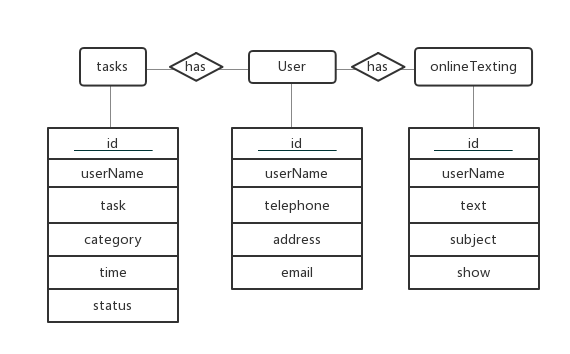
\includegraphics[width=\textwidth]{dt_database}
    \caption{Hybrid desktop database design}
    \label{fig:mesh1}
\end{figure}
\\
Table User is the foundational one. Because each Hybrid Desktop’s data only belongs to one user, so these three table will be connected through the userID (primary key). Each task must have an id, userName, task, category, time, and status. And it will connect with User by userName. Id is an automatically increasing index, time is a time stamp, and will insert by MYSQL program based on the current time. Status will have a default value which is 0 stands for that task has not been finished yet. And the table User is just used for storing the basic information of the user. For the online Texting table, it will connect with User by username. The show property stands for whether this annotation should be displayed in the annotation box or not, and it will have a default value which is 0. Besides, every property in the online texting should not be null.


